\documentclass[../main.tex]{subfiles}

\begin{document}

\subsection{Writing time VS Block size}
\begin{figure}[h]
    \centering
    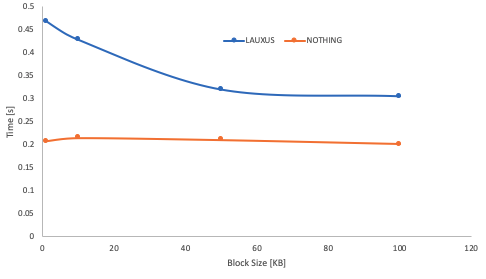
\includegraphics[width=\textwidth]{images/appendix/perf_write_per_block_size}
    
    \caption{A 1KB File writing time VS block size}
    \label{appendix:figure:perf_time_per_block_size}
\end{figure}
\par As we are using a stateless model (no session) for writing the encrypted file to the remote storage, the more we increase the block size, the more we are efficient (to a certain threshold). By stateless model, we just mean that on each write, we open the file on the remote storage. A more efficient approach would be to open the file at the same time the end user opens it. However this should not highly change the performance as the writing time is mainly governed by the encryption time.

\subsection{Block Writing time throughout an entire file write}
\begin{figure}[h]
    \centering
    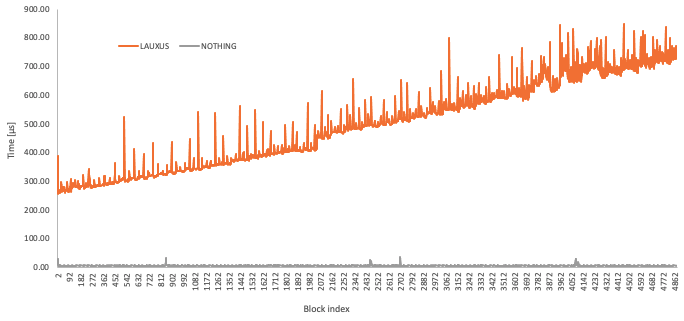
\includegraphics[width=\textwidth]{images/appendix/perf_write_per_block_time}
    
    \caption{Evolution of the block writing time for a 20MB File}
    \label{appendix:figure:perf_time_per_block}
\end{figure}
\par As we can see from the Figure \ref{appendix:figure:perf_time_per_block}, the write time is not constant throughout an full write operation. This explains why we don't have a perfect linear evolution in the Figure \ref{}. The reason for this behaviour is that on every write operation, we are writing the entire metadata structure to the remote storage. We need to do so as we are creating a new content block and thus we must create a new key. As the metadata structure becomes bigger and bigger, it takes more and more time to encrypt and write it. This is way we don't have a constant time.

\end{document}